\documentclass[UTF8]{article}
\usepackage{ctex}
\usepackage{ulem}
\usepackage{amssymb}
\usepackage{amsmath}
\usepackage{graphicx}
\newtheorem{thm}{定义}[section]
\newtheorem{notation}[thm]{记号}
\newtheorem{lemma}[thm]{引理}

\makeatletter
\newcommand{\rmnum}[1]{\romannumeral #1}
\newcommand{\Rmnum}[1]{\expandafter\@slowromancap\romannumeral #1@}
\makeatother
\newcommand{\dperp}{\perp\!\!\!\perp}

\title{11 $\lambda{\rm D}$中Flag风格的自然演绎\\Flag-style natural deduction in $\lambda{\rm D}$\\[2ex]\begin{large}读书笔记\end{large}}
\author{许博}
\date{}

\begin{document}
\maketitle
	\section{$\lambda{\rm D}$中的形式化推导}
	\noindent
	在$\lambda{\rm D}$中,我们可以以更有效更优雅的方式表示逻辑,尤其是构造逻辑。在章节7.1和7.2中,我们遇到了一些$\lambda{\rm C}$中处理逻辑的“隐藏”定义。作为例子,使用$\lambda{rm D}$的标准形式表示下列三者:
	
	\noindent
	\textit{Absurdity}\\
	$\lambda{\rm C}$使用$\perp$表示$\Pi\alpha:*.\alpha$,行为与描述性定义相同,在$\lambda{\rm D}$中可以写作:
	
		$\emptyset\triangleright\perp():=\Pi\alpha:*.\alpha:*$。
		
	\noindent
	\textit{Negation}\\
	之前使用$\neg A$作为$A\rightarrow\perp$的简写,同样也是一个描述性定义:
	
		$A:*\triangleright\neg(A):=A\rightarrow\perp():*$。
	
	\noindent
	\textit{Conjunction}\\
	同样的,我们可以定义合取,具有了两个参数:
	
		$A:*,B:*\triangleright\land(A,B):=\Pi C:*.(A\rightarrow B\rightarrow C)\rightarrow C:*$。
		
		形如以上的逻辑定义在$\lambda{\rm D}$中能够被形式化推导。因为需要先推导出定义实体之后,才能够在环境中添加定义。比如$\neg$的定义的一个$\lambda{\rm D_0}$-推导:\\
		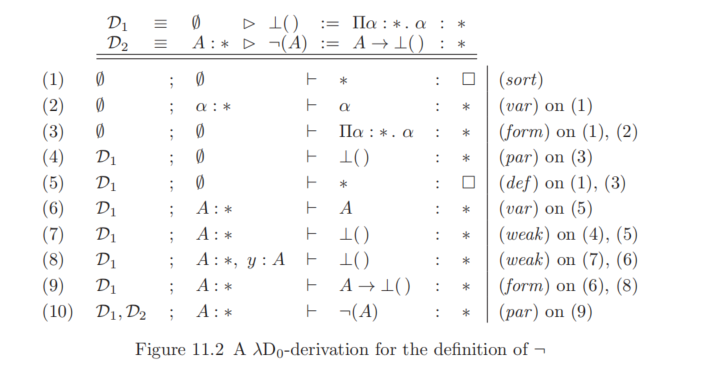
\includegraphics[width=0.93\linewidth]{"../imgs/11-1.png"}
		
		通常来说,推导会从底端开始,也即需要考虑如果能够到达最后的推定。需要从推导规则,不断从$\bf conclusion$反推所需要的$\bf premiss$。
	
	\section{对比形式化和flag-风格的$\lambda{\rm D}$}
	\noindent
	在第四章及以后,我们在推导时,将应用了规则(sort),(var),(weak)以及(form)的步骤省略,以获得更紧凑的推导过程,同时舍去了一些并不有趣的步骤,现在在$\lambda{\rm D}$中,也将这样做,除了上述提到的规则,还加入了规则(def)。
	
		一个有趣的问题是如何使用flag-风格表示图11.2中的线性格式,如下(已经使用了简化版本):\\
		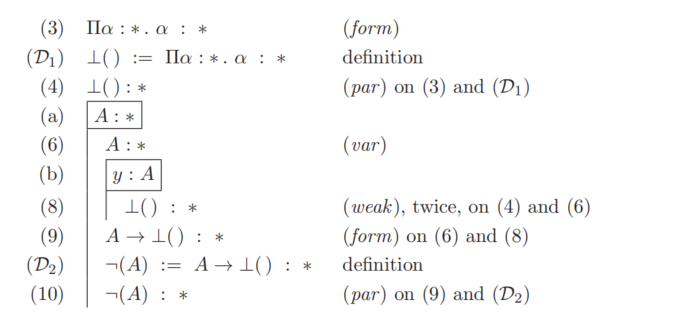
\includegraphics[width=0.93\linewidth]{"../imgs/11-2.png"}
		
		两个版本之间极为相似。而观察行(3)到(4),会发现信息的重复,以及($\mathcal{D}_1$)和行(9)和(10)。看起来只保留($\mathcal{D}_1$)和($\mathcal{D}_2$)而删除行(3),(4),(9)和(10)是非常合理的。
		
		以及行(6)和(8)或多或少都有些多余,行(9)是假设(a)和行(4)的一个显而易见的结果,所以我们可以跳过行(6)和(8),以及假设(b)。
		
		应用了上述修改,得到如下flag-风格的推导:\\
		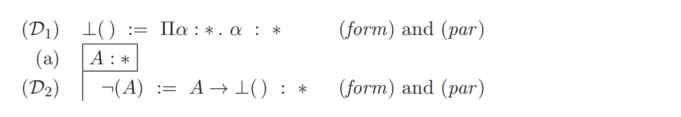
\includegraphics[width=0.93\linewidth]{"../imgs/11-3.png"}
		
		至此,通过重写证明到flag形式,以及省略一些非常明显的行,我们得到了一个flag风格的推导,与在章节11.1开头相对应的定义的表示相同。
\end{document}
